\documentclass[1p]{elsarticle_modified}
%\bibliographystyle{elsarticle-num}

%\usepackage[colorlinks]{hyperref}
%\usepackage{abbrmath_seonhwa} %\Abb, \Ascr, \Acal ,\Abf, \Afrak
\usepackage{amsfonts}
\usepackage{amssymb}
\usepackage{amsmath}
\usepackage{amsthm}
\usepackage{scalefnt}
\usepackage{amsbsy}
\usepackage{kotex}
\usepackage{caption}
\usepackage{subfig}
\usepackage{color}
\usepackage{graphicx}
\usepackage{xcolor} %% white, black, red, green, blue, cyan, magenta, yellow
\usepackage{float}
\usepackage{setspace}
\usepackage{hyperref}

\usepackage{tikz}
\usetikzlibrary{arrows}

\usepackage{multirow}
\usepackage{array} % fixed length table
\usepackage{hhline}

%%%%%%%%%%%%%%%%%%%%%
\makeatletter
\renewcommand*\env@matrix[1][\arraystretch]{%
	\edef\arraystretch{#1}%
	\hskip -\arraycolsep
	\let\@ifnextchar\new@ifnextchar
	\array{*\c@MaxMatrixCols c}}
\makeatother %https://tex.stackexchange.com/questions/14071/how-can-i-increase-the-line-spacing-in-a-matrix
%%%%%%%%%%%%%%%

\usepackage[normalem]{ulem}

\newcommand{\msout}[1]{\ifmmode\text{\sout{\ensuremath{#1}}}\else\sout{#1}\fi}
%SOURCE: \msout is \stkout macro in https://tex.stackexchange.com/questions/20609/strikeout-in-math-mode

\newcommand{\cancel}[1]{
	\ifmmode
	{\color{red}\msout{#1}}
	\else
	{\color{red}\sout{#1}}
	\fi
}

\newcommand{\add}[1]{
	{\color{blue}\uwave{#1}}
}

\newcommand{\replace}[2]{
	\ifmmode
	{\color{red}\msout{#1}}{\color{blue}\uwave{#2}}
	\else
	{\color{red}\sout{#1}}{\color{blue}\uwave{#2}}
	\fi
}

\newcommand{\Sol}{\mathcal{S}} %segment
\newcommand{\D}{D} %diagram
\newcommand{\A}{\mathcal{A}} %arc


%%%%%%%%%%%%%%%%%%%%%%%%%%%%%5 test

\def\sl{\operatorname{\textup{SL}}(2,\Cbb)}
\def\psl{\operatorname{\textup{PSL}}(2,\Cbb)}
\def\quan{\mkern 1mu \triangleright \mkern 1mu}

\theoremstyle{definition}
\newtheorem{thm}{Theorem}[section]
\newtheorem{prop}[thm]{Proposition}
\newtheorem{lem}[thm]{Lemma}
\newtheorem{ques}[thm]{Question}
\newtheorem{cor}[thm]{Corollary}
\newtheorem{defn}[thm]{Definition}
\newtheorem{exam}[thm]{Example}
\newtheorem{rmk}[thm]{Remark}
\newtheorem{alg}[thm]{Algorithm}

\newcommand{\I}{\sqrt{-1}}
\begin{document}

%\begin{frontmatter}
%
%\title{Boundary parabolic representations of knots up to 8 crossings}
%
%%% Group authors per affiliation:
%\author{Yunhi Cho} 
%\address{Department of Mathematics, University of Seoul, Seoul, Korea}
%\ead{yhcho@uos.ac.kr}
%
%
%\author{Seonhwa Kim} %\fnref{s_kim}}
%\address{Center for Geometry and Physics, Institute for Basic Science, Pohang, 37673, Korea}
%\ead{ryeona17@ibs.re.kr}
%
%\author{Hyuk Kim}
%\address{Department of Mathematical Sciences, Seoul National University, Seoul 08826, Korea}
%\ead{hyukkim@snu.ac.kr}
%
%\author{Seokbeom Yoon}
%\address{Department of Mathematical Sciences, Seoul National University, Seoul, 08826,  Korea}
%\ead{sbyoon15@snu.ac.kr}
%
%\begin{abstract}
%We find all boundary parabolic representation of knots up to 8 crossings.
%
%\end{abstract}
%\begin{keyword}
%    \MSC[2010] 57M25 
%\end{keyword}
%
%\end{frontmatter}

%\linenumbers
%\tableofcontents
%
\newcommand\colored[1]{\textcolor{white}{\rule[-0.35ex]{0.8em}{1.4ex}}\kern-0.8em\color{red} #1}%
%\newcommand\colored[1]{\textcolor{white}{ #1}\kern-2.17ex	\textcolor{white}{ #1}\kern-1.81ex	\textcolor{white}{ #1}\kern-2.15ex\color{red}#1	}

{\Large $\underline{12n_{0809}~(K12n_{0809})}$}

\setlength{\tabcolsep}{10pt}
\renewcommand{\arraystretch}{1.6}
\vspace{1cm}\begin{tabular}{m{100pt}>{\centering\arraybackslash}m{274pt}}
\multirow{5}{120pt}{
	\centering
	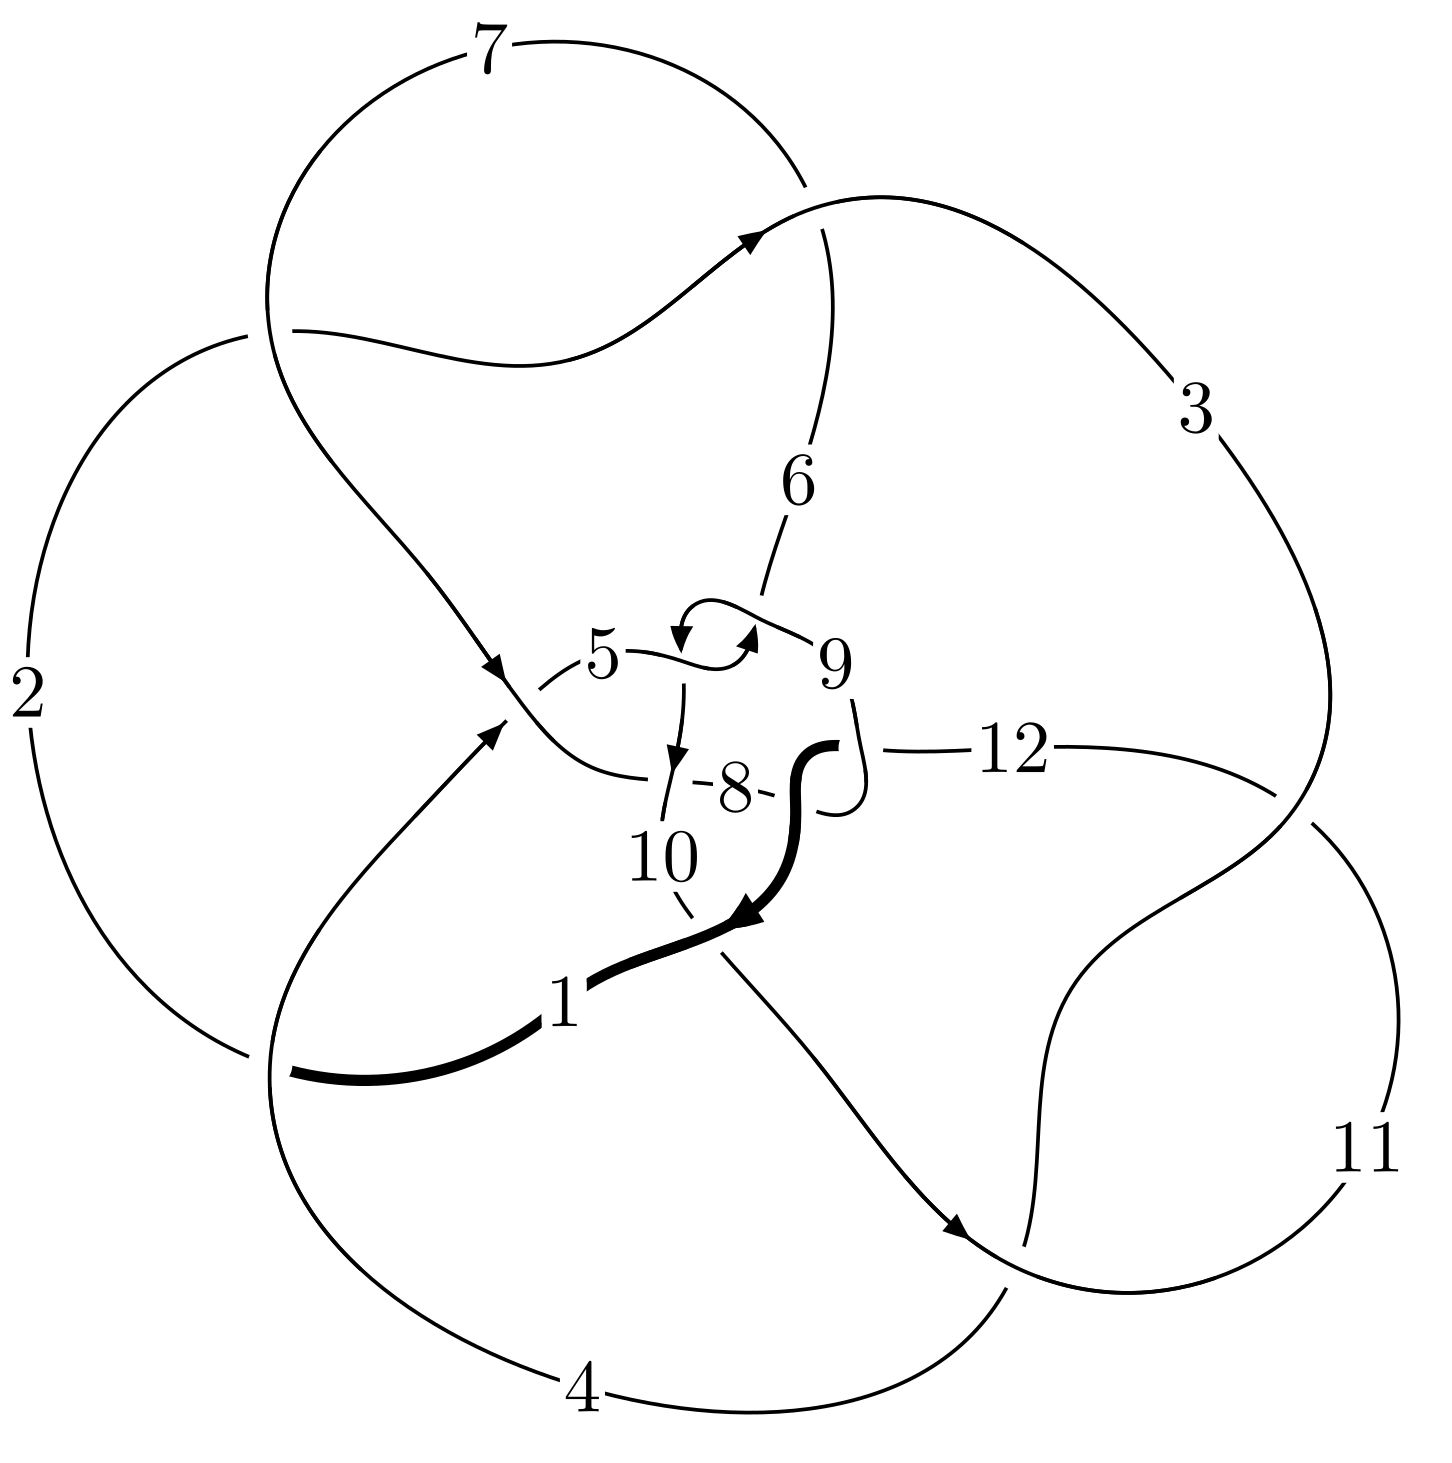
\includegraphics[width=112pt]{../../../GIT/diagram.site/Diagrams/png/2898_12n_0809.png}\\
\ \ \ A knot diagram\footnotemark}&
\allowdisplaybreaks
\textbf{Linearized knot diagam} \\
\cline{2-2}
 &
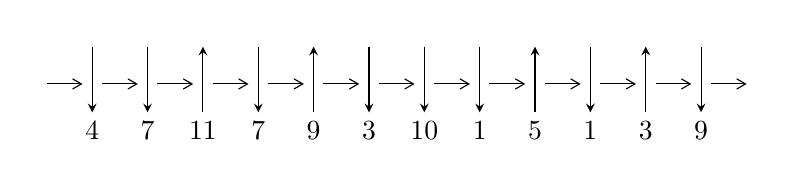
\begin{tikzpicture}[x=20pt, y=17pt]
	% nodes
	\node (C0) at (0, 0) {};
	\node (C1) at (1, 0) {};
	\node (C1U) at (1, +1) {};
	\node (C1D) at (1, -1) {4};

	\node (C2) at (2, 0) {};
	\node (C2U) at (2, +1) {};
	\node (C2D) at (2, -1) {7};

	\node (C3) at (3, 0) {};
	\node (C3U) at (3, +1) {};
	\node (C3D) at (3, -1) {11};

	\node (C4) at (4, 0) {};
	\node (C4U) at (4, +1) {};
	\node (C4D) at (4, -1) {7};

	\node (C5) at (5, 0) {};
	\node (C5U) at (5, +1) {};
	\node (C5D) at (5, -1) {9};

	\node (C6) at (6, 0) {};
	\node (C6U) at (6, +1) {};
	\node (C6D) at (6, -1) {3};

	\node (C7) at (7, 0) {};
	\node (C7U) at (7, +1) {};
	\node (C7D) at (7, -1) {10};

	\node (C8) at (8, 0) {};
	\node (C8U) at (8, +1) {};
	\node (C8D) at (8, -1) {1};

	\node (C9) at (9, 0) {};
	\node (C9U) at (9, +1) {};
	\node (C9D) at (9, -1) {5};

	\node (C10) at (10, 0) {};
	\node (C10U) at (10, +1) {};
	\node (C10D) at (10, -1) {1};

	\node (C11) at (11, 0) {};
	\node (C11U) at (11, +1) {};
	\node (C11D) at (11, -1) {3};

	\node (C12) at (12, 0) {};
	\node (C12U) at (12, +1) {};
	\node (C12D) at (12, -1) {9};
	\node (C13) at (13, 0) {};

	% arrows
	\draw[->,>={angle 60}]
	(C0) edge (C1) (C1) edge (C2) (C2) edge (C3) (C3) edge (C4) (C4) edge (C5) (C5) edge (C6) (C6) edge (C7) (C7) edge (C8) (C8) edge (C9) (C9) edge (C10) (C10) edge (C11) (C11) edge (C12) (C12) edge (C13) ;	\draw[->,>=stealth]
	(C1U) edge (C1D) (C2U) edge (C2D) (C3D) edge (C3U) (C4U) edge (C4D) (C5D) edge (C5U) (C6U) edge (C6D) (C7U) edge (C7D) (C8U) edge (C8D) (C9D) edge (C9U) (C10U) edge (C10D) (C11D) edge (C11U) (C12U) edge (C12D) ;
	\end{tikzpicture} \\
\hhline{~~} \\& 
\textbf{Solving Sequence} \\ \cline{2-2} 
 &
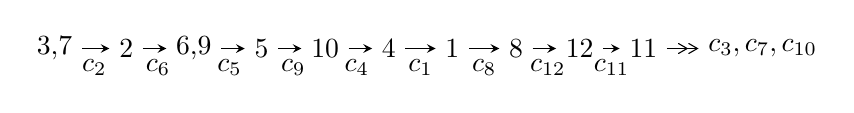
\begin{tikzpicture}[x=23pt, y=7pt]
	% node
	\node (A0) at (-1/8, 0) {3,7};
	\node (A1) at (1, 0) {2};
	\node (A2) at (33/16, 0) {6,9};
	\node (A3) at (25/8, 0) {5};
	\node (A4) at (33/8, 0) {10};
	\node (A5) at (41/8, 0) {4};
	\node (A6) at (49/8, 0) {1};
	\node (A7) at (57/8, 0) {8};
	\node (A8) at (65/8, 0) {12};
	\node (A9) at (73/8, 0) {11};
	\node (C1) at (1/2, -1) {$c_{2}$};
	\node (C2) at (3/2, -1) {$c_{6}$};
	\node (C3) at (21/8, -1) {$c_{5}$};
	\node (C4) at (29/8, -1) {$c_{9}$};
	\node (C5) at (37/8, -1) {$c_{4}$};
	\node (C6) at (45/8, -1) {$c_{1}$};
	\node (C7) at (53/8, -1) {$c_{8}$};
	\node (C8) at (61/8, -1) {$c_{12}$};
	\node (C9) at (69/8, -1) {$c_{11}$};
	\node (A10) at (11, 0) {$c_{3},c_{7},c_{10}$};

	% edge
	\draw[->,>=stealth]	
	(A0) edge (A1) (A1) edge (A2) (A2) edge (A3) (A3) edge (A4) (A4) edge (A5) (A5) edge (A6) (A6) edge (A7) (A7) edge (A8) (A8) edge (A9) ;
	\draw[->>,>={angle 60}]	
	(A9) edge (A10);
\end{tikzpicture} \\ 

\end{tabular} \\

\footnotetext{
The image of knot diagram is generated by the software ``\textbf{Draw programme}" developed by Andrew Bartholomew(\url{http://www.layer8.co.uk/maths/draw/index.htm\#Running-draw}), where we modified some parts for our purpose(\url{https://github.com/CATsTAILs/LinksPainter}).
}\phantom \\ \newline 
\centering \textbf{Ideals for irreducible components\footnotemark of $X_{\text{par}}$} 
 
\begin{align*}
I^u_{1}&=\langle 
571 u^8-2565 u^7+12003 u^6-25350 u^5+52034 u^4-56137 u^3+50704 u^2+9862 b-34468 u+8850,\\
\phantom{I^u_{1}}&\phantom{= \langle  }-257 u^8-1039 u^7+\cdots+19724 a+18176,\\
\phantom{I^u_{1}}&\phantom{= \langle  }u^9-5 u^8+23 u^7-53 u^6+102 u^5-114 u^4+74 u^3-44 u^2+16 u-4\rangle \\
I^u_{2}&=\langle 
a^3-4 a^2+5 b+2 a-3,\;a^4-3 a^3+8 a^2-6 a+7,\;u+1\rangle \\
I^u_{3}&=\langle 
u^3 a-2 u^2 a- u^3-2 a u-3 u^2+5 b-2 a-3 u-3,\;u^3 a-2 u^2 a- u^3+2 a^2-2 a u-5 u^2+4 a-4 u+2,\\
\phantom{I^u_{3}}&\phantom{= \langle  }u^4+2 u^3+2\rangle \\
I^u_{4}&=\langle 
-21 u^5+7 u^4-143 u^3+282 u^2+4 b-318 u+128,\\
\phantom{I^u_{4}}&\phantom{= \langle  }-43 u^5+14 u^4-292 u^3+577 u^2+4 a-644 u+258,\;u^6- u^5+7 u^4-18 u^3+24 u^2-16 u+4\rangle \\
I^u_{5}&=\langle 
2 a u+11 b-16 a- u-3,\;32 a^2+4 a u+8 a+7 u+34,\;u^2+2 u+8\rangle \\
I^u_{6}&=\langle 
b,\;a+u-1,\;u^2- u-1\rangle \\
I^u_{7}&=\langle 
b^2+1,\;a-1,\;u-1\rangle \\
I^u_{8}&=\langle 
b- u+1,\;2 a^2- a u+2 a-1,\;u^2-2 u+2\rangle \\
\\
\end{align*}
\raggedright * 8 irreducible components of $\dim_{\mathbb{C}}=0$, with total 39 representations.\\
\footnotetext{All coefficients of polynomials are rational numbers. But the coefficients are sometimes approximated in decimal forms when there is not enough margin.}
\newpage
\renewcommand{\arraystretch}{1}
\centering \section*{I. $I^u_{1}= \langle 571 u^8-2565 u^7+\cdots+9862 b+8850,\;-257 u^8-1039 u^7+\cdots+19724 a+18176,\;u^9-5 u^8+\cdots+16 u-4 \rangle$}
\flushleft \textbf{(i) Arc colorings}\\
\begin{tabular}{m{7pt} m{180pt} m{7pt} m{180pt} }
\flushright $a_{3}=$&$\begin{pmatrix}1\\0\end{pmatrix}$ \\
\flushright $a_{7}=$&$\begin{pmatrix}0\\u\end{pmatrix}$ \\
\flushright $a_{2}=$&$\begin{pmatrix}1\\- u^2\end{pmatrix}$ \\
\flushright $a_{6}=$&$\begin{pmatrix}u\\u\end{pmatrix}$ \\
\flushright $a_{9}=$&$\begin{pmatrix}0.0130298 u^{8}+0.0526769 u^{7}+\cdots+2.85094 u-0.921517\\-0.0578990 u^{8}+0.260089 u^{7}+\cdots+3.49503 u-0.897384\end{pmatrix}$ \\
\flushright $a_{5}=$&$\begin{pmatrix}-0.0833502 u^{8}+0.342020 u^{7}+\cdots-2.24883 u+1.32286\\-0.0747313 u^{8}+0.411884 u^{7}+\cdots+2.65646 u-0.333401\end{pmatrix}$ \\
\flushright $a_{10}=$&$\begin{pmatrix}0.0833502 u^{8}-0.342020 u^{7}+\cdots+2.24883 u-1.32286\\-0.100994 u^{8}+0.410769 u^{7}+\cdots+1.96857 u-0.616102\end{pmatrix}$ \\
\flushright $a_{4}=$&$\begin{pmatrix}-0.0833502 u^{8}+0.342020 u^{7}+\cdots-2.24883 u+1.32286\\-0.112959 u^{8}+0.560840 u^{7}+\cdots+1.79416 u-0.0344758\end{pmatrix}$ \\
\flushright $a_{1}=$&$\begin{pmatrix}0.0407118 u^{8}-0.175877 u^{7}+\cdots+2.44088 u+0.241330\\0.117826 u^{8}-0.562563 u^{7}+\cdots-1.12999 u+0.0521192\end{pmatrix}$ \\
\flushright $a_{8}=$&$\begin{pmatrix}0.0407118 u^{8}-0.175877 u^{7}+\cdots+2.44088 u-0.758670\\-0.0313324 u^{8}+0.104847 u^{7}+\cdots+1.66193 u-0.426080\end{pmatrix}$ \\
\flushright $a_{12}=$&$\begin{pmatrix}-0.0771142 u^{8}+0.386686 u^{7}+\cdots+3.57088 u+0.189211\\0.147232 u^{8}-0.677145 u^{7}+\cdots-1.15899 u+0.283715\end{pmatrix}$ \\
\flushright $a_{11}=$&$\begin{pmatrix}-0.224346 u^{8}+1.06383 u^{7}+\cdots+4.72987 u-0.0945042\\0.147232 u^{8}-0.677145 u^{7}+\cdots-1.15899 u+0.283715\end{pmatrix}$\\&\end{tabular}
\flushleft \textbf{(ii) Obstruction class $= -1$}\\~\\
\flushleft \textbf{(iii) Cusp Shapes $= -\frac{8556}{4931} u^8+\frac{38780}{4931} u^7-\frac{177291}{4931} u^6+\frac{363598}{4931} u^5-\frac{671631}{4931} u^4+\frac{589646}{4931} u^3-\frac{228370}{4931} u^2+\frac{136712}{4931} u-\frac{48274}{4931}$}\\~\\
\newpage\renewcommand{\arraystretch}{1}
\flushleft \textbf{(iv) u-Polynomials at the component}\newline \\
\begin{tabular}{m{50pt}|m{274pt}}
Crossings & \hspace{64pt}u-Polynomials at each crossing \\
\hline $$\begin{aligned}c_{1},c_{4},c_{7}\\c_{10}\end{aligned}$$&$\begin{aligned}
&u^9-2 u^8-4 u^7+11 u^6+6 u^5-16 u^4-5 u^3+8 u^2+2 u+1
\end{aligned}$\\
\hline $$\begin{aligned}c_{2},c_{6},c_{8}\\c_{12}\end{aligned}$$&$\begin{aligned}
&u^9+5 u^8+23 u^7+53 u^6+102 u^5+114 u^4+74 u^3+44 u^2+16 u+4
\end{aligned}$\\
\hline $$\begin{aligned}c_{3},c_{5},c_{9}\\c_{11}\end{aligned}$$&$\begin{aligned}
&u^9-3 u^8+2 u^7+5 u^6+2 u^5-9 u^4+25 u^3-18 u^2+8 u-2
\end{aligned}$\\
\hline
\end{tabular}\\~\\
\newpage\renewcommand{\arraystretch}{1}
\flushleft \textbf{(v) Riley Polynomials at the component}\newline \\
\begin{tabular}{m{50pt}|m{274pt}}
Crossings & \hspace{64pt}Riley Polynomials at each crossing \\
\hline $$\begin{aligned}c_{1},c_{4},c_{7}\\c_{10}\end{aligned}$$&$\begin{aligned}
&y^9-12 y^8+\cdots-12 y-1
\end{aligned}$\\
\hline $$\begin{aligned}c_{2},c_{6},c_{8}\\c_{12}\end{aligned}$$&$\begin{aligned}
&y^9+21 y^8+\cdots-96 y-16
\end{aligned}$\\
\hline $$\begin{aligned}c_{3},c_{5},c_{9}\\c_{11}\end{aligned}$$&$\begin{aligned}
&y^9-5 y^8+38 y^7-21 y^6+102 y^5+219 y^4+353 y^3+40 y^2-8 y-4
\end{aligned}$\\
\hline
\end{tabular}\\~\\
\newpage\flushleft \textbf{(vi) Complex Volumes and Cusp Shapes}
$$\begin{array}{c|c|c}  
\text{Solutions to }I^u_{1}& \I (\text{vol} + \sqrt{-1}CS) & \text{Cusp shape}\\
 \hline 
\begin{aligned}
u &= \phantom{-}1.12609\phantom{ +0.000000I} \\
a &= -0.807283\phantom{ +0.000000I} \\
b &= -1.21689\phantom{ +0.000000I}\end{aligned}
 & -7.72540\phantom{ +0.000000I} & -11.7840\phantom{ +0.000000I} \\ \hline\begin{aligned}
u &= -0.041387 + 0.594605 I \\
a &= \phantom{-}2.03957 + 0.32064 I \\
b &= \phantom{-}0.362527 + 1.166500 I\end{aligned}
 & -3.87094 + 3.77664 I & -6.27308 - 5.05750 I \\ \hline\begin{aligned}
u &= -0.041387 - 0.594605 I \\
a &= \phantom{-}2.03957 - 0.32064 I \\
b &= \phantom{-}0.362527 - 1.166500 I\end{aligned}
 & -3.87094 - 3.77664 I & -6.27308 + 5.05750 I \\ \hline\begin{aligned}
u &= \phantom{-}0.320133 + 0.346415 I \\
a &= -0.384796 - 0.492791 I \\
b &= \phantom{-}0.064812 + 0.443428 I\end{aligned}
 & -0.209220 - 0.942065 I & -4.31920 + 7.08722 I \\ \hline\begin{aligned}
u &= \phantom{-}0.320133 - 0.346415 I \\
a &= -0.384796 + 0.492791 I \\
b &= \phantom{-}0.064812 - 0.443428 I\end{aligned}
 & -0.209220 + 0.942065 I & -4.31920 - 7.08722 I \\ \hline\begin{aligned}
u &= \phantom{-}0.54446 + 2.21567 I \\
a &= \phantom{-}0.180263 - 1.209750 I \\
b &= -0.03727 - 1.87202 I\end{aligned}
 & \phantom{-}9.45113 - 2.91184 I & -5.37168 + 2.28602 I \\ \hline\begin{aligned}
u &= \phantom{-}0.54446 - 2.21567 I \\
a &= \phantom{-}0.180263 + 1.209750 I \\
b &= -0.03727 + 1.87202 I\end{aligned}
 & \phantom{-}9.45113 + 2.91184 I & -5.37168 - 2.28602 I \\ \hline\begin{aligned}
u &= \phantom{-}1.11375 + 2.71889 I \\
a &= \phantom{-}0.068603 + 1.166970 I \\
b &= \phantom{-}0.21838 + 1.96553 I\end{aligned}
 & \phantom{-}5.89393 - 11.43930 I & -5.14383 + 4.44122 I \\ \hline\begin{aligned}
u &= \phantom{-}1.11375 - 2.71889 I \\
a &= \phantom{-}0.068603 - 1.166970 I \\
b &= \phantom{-}0.21838 - 1.96553 I\end{aligned}
 & \phantom{-}5.89393 + 11.43930 I & -5.14383 - 4.44122 I\\
 \hline 
 \end{array}$$\newpage\newpage\renewcommand{\arraystretch}{1}
\centering \section*{II. $I^u_{2}= \langle a^3-4 a^2+5 b+2 a-3,\;a^4-3 a^3+8 a^2-6 a+7,\;u+1 \rangle$}
\flushleft \textbf{(i) Arc colorings}\\
\begin{tabular}{m{7pt} m{180pt} m{7pt} m{180pt} }
\flushright $a_{3}=$&$\begin{pmatrix}1\\0\end{pmatrix}$ \\
\flushright $a_{7}=$&$\begin{pmatrix}0\\-1\end{pmatrix}$ \\
\flushright $a_{2}=$&$\begin{pmatrix}1\\-1\end{pmatrix}$ \\
\flushright $a_{6}=$&$\begin{pmatrix}-1\\-1\end{pmatrix}$ \\
\flushright $a_{9}=$&$\begin{pmatrix}a\\-\frac{1}{5} a^3+\frac{4}{5} a^2-\frac{2}{5} a+\frac{3}{5}\end{pmatrix}$ \\
\flushright $a_{5}=$&$\begin{pmatrix}-\frac{1}{5} a^3-\frac{1}{5} a^2+\frac{3}{5} a-\frac{12}{5}\\-\frac{2}{5} a^3+\frac{3}{5} a^2-\frac{4}{5} a-\frac{4}{5}\end{pmatrix}$ \\
\flushright $a_{10}=$&$\begin{pmatrix}-\frac{2}{5} a^3+\frac{3}{5} a^2-\frac{4}{5} a-\frac{4}{5}\\-\frac{3}{5} a^3+\frac{7}{5} a^2-\frac{11}{5} a+\frac{4}{5}\end{pmatrix}$ \\
\flushright $a_{4}=$&$\begin{pmatrix}-\frac{1}{5} a^3-\frac{1}{5} a^2+\frac{3}{5} a-\frac{12}{5}\\-\frac{1}{5} a^3+\frac{4}{5} a^2-\frac{7}{5} a+\frac{8}{5}\end{pmatrix}$ \\
\flushright $a_{1}=$&$\begin{pmatrix}\frac{1}{5} a^3-\frac{4}{5} a^2+\frac{7}{5} a-\frac{13}{5}\\- a\end{pmatrix}$ \\
\flushright $a_{8}=$&$\begin{pmatrix}-\frac{1}{5} a^3+\frac{4}{5} a^2-\frac{2}{5} a+\frac{13}{5}\\-\frac{1}{5} a^3+\frac{4}{5} a^2+\frac{3}{5} a+\frac{3}{5}\end{pmatrix}$ \\
\flushright $a_{12}=$&$\begin{pmatrix}\frac{1}{5} a^3-\frac{4}{5} a^2+\frac{12}{5} a-\frac{13}{5}\\-\frac{1}{5} a^3+\frac{4}{5} a^2-\frac{7}{5} a+\frac{3}{5}\end{pmatrix}$ \\
\flushright $a_{11}=$&$\begin{pmatrix}\frac{2}{5} a^3-\frac{8}{5} a^2+\frac{19}{5} a-\frac{16}{5}\\-\frac{1}{5} a^3+\frac{4}{5} a^2-\frac{7}{5} a+\frac{3}{5}\end{pmatrix}$\\&\end{tabular}
\flushleft \textbf{(ii) Obstruction class $= -1$}\\~\\
\flushleft \textbf{(iii) Cusp Shapes $= -\frac{8}{5} a^3+\frac{32}{5} a^2-\frac{56}{5} a-\frac{26}{5}$}\\~\\
\newpage\renewcommand{\arraystretch}{1}
\flushleft \textbf{(iv) u-Polynomials at the component}\newline \\
\begin{tabular}{m{50pt}|m{274pt}}
Crossings & \hspace{64pt}u-Polynomials at each crossing \\
\hline $$\begin{aligned}c_{1},c_{4},c_{7}\\c_{10}\end{aligned}$$&$\begin{aligned}
&u^4+u^3-4 u^2-4 u+7
\end{aligned}$\\
\hline $$\begin{aligned}c_{2},c_{6},c_{8}\\c_{12}\end{aligned}$$&$\begin{aligned}
&(u-1)^4
\end{aligned}$\\
\hline $$\begin{aligned}c_{3},c_{5},c_{9}\\c_{11}\end{aligned}$$&$\begin{aligned}
&(u^2+u+1)^2
\end{aligned}$\\
\hline
\end{tabular}\\~\\
\newpage\renewcommand{\arraystretch}{1}
\flushleft \textbf{(v) Riley Polynomials at the component}\newline \\
\begin{tabular}{m{50pt}|m{274pt}}
Crossings & \hspace{64pt}Riley Polynomials at each crossing \\
\hline $$\begin{aligned}c_{1},c_{4},c_{7}\\c_{10}\end{aligned}$$&$\begin{aligned}
&y^4-9 y^3+38 y^2-72 y+49
\end{aligned}$\\
\hline $$\begin{aligned}c_{2},c_{6},c_{8}\\c_{12}\end{aligned}$$&$\begin{aligned}
&(y-1)^4
\end{aligned}$\\
\hline $$\begin{aligned}c_{3},c_{5},c_{9}\\c_{11}\end{aligned}$$&$\begin{aligned}
&(y^2+y+1)^2
\end{aligned}$\\
\hline
\end{tabular}\\~\\
\newpage\flushleft \textbf{(vi) Complex Volumes and Cusp Shapes}
$$\begin{array}{c|c|c}  
\text{Solutions to }I^u_{2}& \I (\text{vol} + \sqrt{-1}CS) & \text{Cusp shape}\\
 \hline 
\begin{aligned}
u &= -1.00000\phantom{ +0.000000I} \\
a &= \phantom{-}0.257518 + 1.105670 I \\
b &= -0.242482 + 0.239643 I\end{aligned}
 & -8.22467 + 4.05977 I & -14.0000 - 6.9282 I \\ \hline\begin{aligned}
u &= -1.00000\phantom{ +0.000000I} \\
a &= \phantom{-}0.257518 - 1.105670 I \\
b &= -0.242482 - 0.239643 I\end{aligned}
 & -8.22467 - 4.05977 I & -14.0000 + 6.9282 I \\ \hline\begin{aligned}
u &= -1.00000\phantom{ +0.000000I} \\
a &= \phantom{-}1.24248 + 1.97169 I \\
b &= \phantom{-}0.74248 + 2.83772 I\end{aligned}
 & -8.22467 - 4.05977 I & -14.0000 + 6.9282 I \\ \hline\begin{aligned}
u &= -1.00000\phantom{ +0.000000I} \\
a &= \phantom{-}1.24248 - 1.97169 I \\
b &= \phantom{-}0.74248 - 2.83772 I\end{aligned}
 & -8.22467 + 4.05977 I & -14.0000 - 6.9282 I\\
 \hline 
 \end{array}$$\newpage\newpage\renewcommand{\arraystretch}{1}
\centering \section*{III. $I^u_{3}= \langle u^3 a- u^3+\cdots-2 a-3,\;u^3 a- u^3+\cdots+4 a+2,\;u^4+2 u^3+2 \rangle$}
\flushleft \textbf{(i) Arc colorings}\\
\begin{tabular}{m{7pt} m{180pt} m{7pt} m{180pt} }
\flushright $a_{3}=$&$\begin{pmatrix}1\\0\end{pmatrix}$ \\
\flushright $a_{7}=$&$\begin{pmatrix}0\\u\end{pmatrix}$ \\
\flushright $a_{2}=$&$\begin{pmatrix}1\\- u^2\end{pmatrix}$ \\
\flushright $a_{6}=$&$\begin{pmatrix}u\\u\end{pmatrix}$ \\
\flushright $a_{9}=$&$\begin{pmatrix}a\\-\frac{1}{5} u^3 a+\frac{1}{5} u^3+\cdots+\frac{2}{5} a+\frac{3}{5}\end{pmatrix}$ \\
\flushright $a_{5}=$&$\begin{pmatrix}\frac{4}{5} u^3 a-\frac{3}{10} u^3+\cdots+\frac{7}{5} a+\frac{3}{5}\\\frac{6}{5} u^3 a-\frac{1}{5} u^3+\cdots+\frac{8}{5} a+\frac{2}{5}\end{pmatrix}$ \\
\flushright $a_{10}=$&$\begin{pmatrix}\frac{1}{5} u^3 a+\frac{3}{10} u^3+\cdots+\frac{3}{5} a+\frac{7}{5}\\\frac{3}{5} u^3 a+\frac{7}{5} u^3+\cdots+\frac{4}{5} a+\frac{6}{5}\end{pmatrix}$ \\
\flushright $a_{4}=$&$\begin{pmatrix}\frac{4}{5} u^3 a-\frac{3}{10} u^3+\cdots+\frac{7}{5} a+\frac{3}{5}\\-\frac{3}{5} u^3 a-\frac{7}{5} u^3+\cdots-\frac{4}{5} a-\frac{6}{5}\end{pmatrix}$ \\
\flushright $a_{1}=$&$\begin{pmatrix}\frac{1}{2} u^3+u^2+u\\- u^3+a u+2 u-1\end{pmatrix}$ \\
\flushright $a_{8}=$&$\begin{pmatrix}u^3+2 u^2+a+u+1\\\frac{4}{5} u^3 a+\frac{6}{5} u^3+\cdots+\frac{12}{5} a+\frac{13}{5}\end{pmatrix}$ \\
\flushright $a_{12}=$&$\begin{pmatrix}u^3 a+u^2 a+\frac{1}{2} u^3- a u+u^2+u\\\frac{4}{5} u^3 a-\frac{4}{5} u^3+\cdots+\frac{2}{5} a-\frac{7}{5}\end{pmatrix}$ \\
\flushright $a_{11}=$&$\begin{pmatrix}\frac{1}{5} u^3 a+\frac{13}{10} u^3+\cdots-\frac{2}{5} a+\frac{7}{5}\\\frac{4}{5} u^3 a-\frac{4}{5} u^3+\cdots+\frac{2}{5} a-\frac{7}{5}\end{pmatrix}$\\&\end{tabular}
\flushleft \textbf{(ii) Obstruction class $= 1$}\\~\\
\flushleft \textbf{(iii) Cusp Shapes $= -2 u^3-2 u^2-6$}\\~\\
\newpage\renewcommand{\arraystretch}{1}
\flushleft \textbf{(iv) u-Polynomials at the component}\newline \\
\begin{tabular}{m{50pt}|m{274pt}}
Crossings & \hspace{64pt}u-Polynomials at each crossing \\
\hline $$\begin{aligned}c_{1},c_{4},c_{7}\\c_{10}\end{aligned}$$&$\begin{aligned}
&u^8-6 u^7+10 u^6+10 u^5-49 u^4+38 u^3+36 u^2-68 u+29
\end{aligned}$\\
\hline $$\begin{aligned}c_{2},c_{8}\end{aligned}$$&$\begin{aligned}
&(u^4+2 u^3+2)^2
\end{aligned}$\\
\hline $$\begin{aligned}c_{3},c_{9}\end{aligned}$$&$\begin{aligned}
&(u^4+u^2-2 u+1)^2
\end{aligned}$\\
\hline $$\begin{aligned}c_{5},c_{11}\end{aligned}$$&$\begin{aligned}
&(u^4+u^2+2 u+1)^2
\end{aligned}$\\
\hline $$\begin{aligned}c_{6},c_{12}\end{aligned}$$&$\begin{aligned}
&(u^4-2 u^3+2)^2
\end{aligned}$\\
\hline
\end{tabular}\\~\\
\newpage\renewcommand{\arraystretch}{1}
\flushleft \textbf{(v) Riley Polynomials at the component}\newline \\
\begin{tabular}{m{50pt}|m{274pt}}
Crossings & \hspace{64pt}Riley Polynomials at each crossing \\
\hline $$\begin{aligned}c_{1},c_{4},c_{7}\\c_{10}\end{aligned}$$&$\begin{aligned}
&y^8-16 y^7+\cdots-2536 y+841
\end{aligned}$\\
\hline $$\begin{aligned}c_{2},c_{6},c_{8}\\c_{12}\end{aligned}$$&$\begin{aligned}
&(y^4-4 y^3+4 y^2+4)^2
\end{aligned}$\\
\hline $$\begin{aligned}c_{3},c_{5},c_{9}\\c_{11}\end{aligned}$$&$\begin{aligned}
&(y^4+2 y^3+3 y^2-2 y+1)^2
\end{aligned}$\\
\hline
\end{tabular}\\~\\
\newpage\flushleft \textbf{(vi) Complex Volumes and Cusp Shapes}
$$\begin{array}{c|c|c}  
\text{Solutions to }I^u_{3}& \I (\text{vol} + \sqrt{-1}CS) & \text{Cusp shape}\\
 \hline 
\begin{aligned}
u &= \phantom{-}0.529086 + 0.742934 I \\
a &= -1.62610 - 0.66493 I \\
b &= -0.067502 - 0.395968 I\end{aligned}
 & -7.40220 + 3.66386 I & -4.00000 - 2.00000 I \\ \hline\begin{aligned}
u &= \phantom{-}0.529086 + 0.742934 I \\
a &= \phantom{-}0.24716 + 2.08709 I \\
b &= -0.41837 + 2.45414 I\end{aligned}
 & -7.40220 + 3.66386 I & -4.00000 - 2.00000 I \\ \hline\begin{aligned}
u &= \phantom{-}0.529086 - 0.742934 I \\
a &= -1.62610 + 0.66493 I \\
b &= -0.067502 + 0.395968 I\end{aligned}
 & -7.40220 - 3.66386 I & -4.00000 + 2.00000 I \\ \hline\begin{aligned}
u &= \phantom{-}0.529086 - 0.742934 I \\
a &= \phantom{-}0.24716 - 2.08709 I \\
b &= -0.41837 - 2.45414 I\end{aligned}
 & -7.40220 - 3.66386 I & -4.00000 + 2.00000 I \\ \hline\begin{aligned}
u &= -1.52909 + 0.25707 I \\
a &= -0.297780 + 0.138203 I \\
b &= \phantom{-}0.067502 + 0.395968 I\end{aligned}
 & -7.40220 + 3.66386 I & -4.00000 - 2.00000 I \\ \hline\begin{aligned}
u &= -1.52909 + 0.25707 I \\
a &= \phantom{-}0.67672 - 1.56036 I \\
b &= \phantom{-}0.41837 - 2.45414 I\end{aligned}
 & -7.40220 + 3.66386 I & -4.00000 - 2.00000 I \\ \hline\begin{aligned}
u &= -1.52909 - 0.25707 I \\
a &= -0.297780 - 0.138203 I \\
b &= \phantom{-}0.067502 - 0.395968 I\end{aligned}
 & -7.40220 - 3.66386 I & -4.00000 + 2.00000 I \\ \hline\begin{aligned}
u &= -1.52909 - 0.25707 I \\
a &= \phantom{-}0.67672 + 1.56036 I \\
b &= \phantom{-}0.41837 + 2.45414 I\end{aligned}
 & -7.40220 - 3.66386 I & -4.00000 + 2.00000 I\\
 \hline 
 \end{array}$$\newpage\newpage\renewcommand{\arraystretch}{1}
\centering \section*{IV. $I^u_{4}= \langle -21 u^5+7 u^4+\cdots+4 b+128,\;-43 u^5+14 u^4+\cdots+4 a+258,\;u^6- u^5+7 u^4-18 u^3+24 u^2-16 u+4 \rangle$}
\flushleft \textbf{(i) Arc colorings}\\
\begin{tabular}{m{7pt} m{180pt} m{7pt} m{180pt} }
\flushright $a_{3}=$&$\begin{pmatrix}1\\0\end{pmatrix}$ \\
\flushright $a_{7}=$&$\begin{pmatrix}0\\u\end{pmatrix}$ \\
\flushright $a_{2}=$&$\begin{pmatrix}1\\- u^2\end{pmatrix}$ \\
\flushright $a_{6}=$&$\begin{pmatrix}u\\u\end{pmatrix}$ \\
\flushright $a_{9}=$&$\begin{pmatrix}\frac{43}{4} u^5-\frac{7}{2} u^4+\cdots+161 u-\frac{129}{2}\\\frac{21}{4} u^5-\frac{7}{4} u^4+\cdots+\frac{159}{2} u-32\end{pmatrix}$ \\
\flushright $a_{5}=$&$\begin{pmatrix}-3 u^5+\frac{5}{4} u^4+\cdots-47 u+\frac{41}{2}\\-\frac{7}{4} u^5+\frac{3}{4} u^4+\cdots-\frac{55}{2} u+12\end{pmatrix}$ \\
\flushright $a_{10}=$&$\begin{pmatrix}4 u^5-\frac{5}{4} u^4+\cdots+60 u-\frac{49}{2}\\\frac{3}{4} u^5-\frac{1}{4} u^4+\cdots+\frac{23}{2} u-5\end{pmatrix}$ \\
\flushright $a_{4}=$&$\begin{pmatrix}-3 u^5+\frac{5}{4} u^4+\cdots-47 u+\frac{41}{2}\\-\frac{3}{4} u^5+\frac{1}{4} u^4+\cdots-\frac{23}{2} u+5\end{pmatrix}$ \\
\flushright $a_{1}=$&$\begin{pmatrix}7 u^5-\frac{11}{4} u^4+\cdots+\frac{217}{2} u-\frac{89}{2}\\\frac{7}{4} u^5-\frac{3}{4} u^4+\cdots+\frac{53}{2} u-11\end{pmatrix}$ \\
\flushright $a_{8}=$&$\begin{pmatrix}\frac{1}{4} u^4+\frac{1}{4} u^3+\cdots-\frac{3}{2} u+\frac{1}{2}\\-\frac{1}{4} u^5+\frac{1}{4} u^4+\cdots-\frac{5}{2} u+1\end{pmatrix}$ \\
\flushright $a_{12}=$&$\begin{pmatrix}\frac{47}{4} u^5-4 u^4+\cdots+177 u-\frac{141}{2}\\\frac{15}{4} u^5-\frac{5}{4} u^4+\cdots+\frac{111}{2} u-22\end{pmatrix}$ \\
\flushright $a_{11}=$&$\begin{pmatrix}8 u^5-\frac{11}{4} u^4+\cdots+\frac{243}{2} u-\frac{97}{2}\\\frac{15}{4} u^5-\frac{5}{4} u^4+\cdots+\frac{111}{2} u-22\end{pmatrix}$\\&\end{tabular}
\flushleft \textbf{(ii) Obstruction class $= 1$}\\~\\
\flushleft \textbf{(iii) Cusp Shapes $= -12 u^5+4 u^4-81 u^3+162 u^2-178 u+68$}\\~\\
\newpage\renewcommand{\arraystretch}{1}
\flushleft \textbf{(iv) u-Polynomials at the component}\newline \\
\begin{tabular}{m{50pt}|m{274pt}}
Crossings & \hspace{64pt}u-Polynomials at each crossing \\
\hline $$\begin{aligned}c_{1},c_{4},c_{7}\\c_{10}\end{aligned}$$&$\begin{aligned}
&u^6- u^5-3 u^3+4 u^2- u+1
\end{aligned}$\\
\hline $$\begin{aligned}c_{2},c_{8}\end{aligned}$$&$\begin{aligned}
&u^6- u^5+7 u^4-18 u^3+24 u^2-16 u+4
\end{aligned}$\\
\hline $$\begin{aligned}c_{3},c_{9}\end{aligned}$$&$\begin{aligned}
&(u^3+2 u^2+1)^2
\end{aligned}$\\
\hline $$\begin{aligned}c_{5},c_{11}\end{aligned}$$&$\begin{aligned}
&(u^3-2 u^2-1)^2
\end{aligned}$\\
\hline $$\begin{aligned}c_{6},c_{12}\end{aligned}$$&$\begin{aligned}
&u^6+u^5+7 u^4+18 u^3+24 u^2+16 u+4
\end{aligned}$\\
\hline
\end{tabular}\\~\\
\newpage\renewcommand{\arraystretch}{1}
\flushleft \textbf{(v) Riley Polynomials at the component}\newline \\
\begin{tabular}{m{50pt}|m{274pt}}
Crossings & \hspace{64pt}Riley Polynomials at each crossing \\
\hline $$\begin{aligned}c_{1},c_{4},c_{7}\\c_{10}\end{aligned}$$&$\begin{aligned}
&y^6- y^5+2 y^4-9 y^3+10 y^2+7 y+1
\end{aligned}$\\
\hline $$\begin{aligned}c_{2},c_{6},c_{8}\\c_{12}\end{aligned}$$&$\begin{aligned}
&y^6+13 y^5+61 y^4-12 y^3+56 y^2-64 y+16
\end{aligned}$\\
\hline $$\begin{aligned}c_{3},c_{5},c_{9}\\c_{11}\end{aligned}$$&$\begin{aligned}
&(y^3-4 y^2-4 y-1)^2
\end{aligned}$\\
\hline
\end{tabular}\\~\\
\newpage\flushleft \textbf{(vi) Complex Volumes and Cusp Shapes}
$$\begin{array}{c|c|c}  
\text{Solutions to }I^u_{4}& \I (\text{vol} + \sqrt{-1}CS) & \text{Cusp shape}\\
 \hline 
\begin{aligned}
u &= \phantom{-}0.670142 + 0.830077 I \\
a &= -0.756371 + 0.536766 I \\
b &= -0.331547 + 1.003560 I\end{aligned}
 & -2.68183 - 2.56897 I & -2.87609 + 2.13317 I \\ \hline\begin{aligned}
u &= \phantom{-}0.670142 - 0.830077 I \\
a &= -0.756371 - 0.536766 I \\
b &= -0.331547 - 1.003560 I\end{aligned}
 & -2.68183 + 2.56897 I & -2.87609 - 2.13317 I \\ \hline\begin{aligned}
u &= \phantom{-}0.659342 + 0.027822 I \\
a &= \phantom{-}0.52967 + 2.00448 I \\
b &= \phantom{-}0.331547 + 1.003560 I\end{aligned}
 & -2.68183 + 2.56897 I & -2.87609 - 2.13317 I \\ \hline\begin{aligned}
u &= \phantom{-}0.659342 - 0.027822 I \\
a &= \phantom{-}0.52967 - 2.00448 I \\
b &= \phantom{-}0.331547 - 1.003560 I\end{aligned}
 & -2.68183 - 2.56897 I & -2.87609 + 2.13317 I \\ \hline\begin{aligned}
u &= -0.82948 + 2.71700 I \\
a &= \phantom{-}0.226699 - 1.047850 I \\
b &= \phantom{-0.000000 } -1.79041 I\end{aligned}
 & \phantom{-}11.9434\phantom{ +0.000000I} &                  -6
-1.247828 + 0. 10   I\phantom{ +0.000000I} \\ \hline\begin{aligned}
u &= -0.82948 - 2.71700 I \\
a &= \phantom{-}0.226699 + 1.047850 I \\
b &= \phantom{-0.000000 -}1.79041 I\end{aligned}
 & \phantom{-}11.9434\phantom{ +0.000000I} &                  -6
-1.247828 + 0. 10   I\phantom{ +0.000000I}\\
 \hline 
 \end{array}$$\newpage\newpage\renewcommand{\arraystretch}{1}
\centering \section*{V. $I^u_{5}= \langle 2 a u+11 b-16 a- u-3,\;32 a^2+4 a u+8 a+7 u+34,\;u^2+2 u+8 \rangle$}
\flushleft \textbf{(i) Arc colorings}\\
\begin{tabular}{m{7pt} m{180pt} m{7pt} m{180pt} }
\flushright $a_{3}=$&$\begin{pmatrix}1\\0\end{pmatrix}$ \\
\flushright $a_{7}=$&$\begin{pmatrix}0\\u\end{pmatrix}$ \\
\flushright $a_{2}=$&$\begin{pmatrix}1\\2 u+8\end{pmatrix}$ \\
\flushright $a_{6}=$&$\begin{pmatrix}u\\u\end{pmatrix}$ \\
\flushright $a_{9}=$&$\begin{pmatrix}a\\-0.181818 a u+1.45455 a+0.0909091 u+0.272727\end{pmatrix}$ \\
\flushright $a_{5}=$&$\begin{pmatrix}-0.0909091 a u-0.272727 a+0.170455 u-0.113636\\0.0909091 a u-0.727273 a-0.545455 u-1.63636\end{pmatrix}$ \\
\flushright $a_{10}=$&$\begin{pmatrix}-0.0909091 a u-0.272727 a-0.0795455 u-0.613636\\-1.36364 a u+2.90909 a+1.18182 u+2.54545\end{pmatrix}$ \\
\flushright $a_{4}=$&$\begin{pmatrix}-0.0909091 a u-0.272727 a+0.170455 u-0.113636\\-0.818182 a u-1.45455 a-0.0909091 u-5.27273\end{pmatrix}$ \\
\flushright $a_{1}=$&$\begin{pmatrix}\frac{1}{8} u+\frac{1}{4}\\-0.636364 a u-2.90909 a-0.181818 u+0.454545\end{pmatrix}$ \\
\flushright $a_{8}=$&$\begin{pmatrix}a-\frac{1}{4} u+\frac{1}{2}\\2.72727 a u+2.18182 a-0.363636 u-2.09091\end{pmatrix}$ \\
\flushright $a_{12}=$&$\begin{pmatrix}a u+2 a+\frac{1}{8} u+\frac{1}{4}\\0.818182 a u+1.45455 a+0.0909091 u+0.272727\end{pmatrix}$ \\
\flushright $a_{11}=$&$\begin{pmatrix}0.181818 a u+0.545455 a+0.0340909 u-0.0227273\\0.818182 a u+1.45455 a+0.0909091 u+0.272727\end{pmatrix}$\\&\end{tabular}
\flushleft \textbf{(ii) Obstruction class $= -1$}\\~\\
\flushleft \textbf{(iii) Cusp Shapes $= -6$}\\~\\
\newpage\renewcommand{\arraystretch}{1}
\flushleft \textbf{(iv) u-Polynomials at the component}\newline \\
\begin{tabular}{m{50pt}|m{274pt}}
Crossings & \hspace{64pt}u-Polynomials at each crossing \\
\hline $$\begin{aligned}c_{1},c_{4},c_{7}\\c_{10}\end{aligned}$$&$\begin{aligned}
&u^4-4 u^3+11 u^2-14 u+7
\end{aligned}$\\
\hline $$\begin{aligned}c_{2},c_{6},c_{8}\\c_{12}\end{aligned}$$&$\begin{aligned}
&(u^2-2 u+8)^2
\end{aligned}$\\
\hline $$\begin{aligned}c_{3},c_{5},c_{9}\\c_{11}\end{aligned}$$&$\begin{aligned}
&(u^2- u-5)^2
\end{aligned}$\\
\hline
\end{tabular}\\~\\
\newpage\renewcommand{\arraystretch}{1}
\flushleft \textbf{(v) Riley Polynomials at the component}\newline \\
\begin{tabular}{m{50pt}|m{274pt}}
Crossings & \hspace{64pt}Riley Polynomials at each crossing \\
\hline $$\begin{aligned}c_{1},c_{4},c_{7}\\c_{10}\end{aligned}$$&$\begin{aligned}
&y^4+6 y^3+23 y^2-42 y+49
\end{aligned}$\\
\hline $$\begin{aligned}c_{2},c_{6},c_{8}\\c_{12}\end{aligned}$$&$\begin{aligned}
&(y^2+12 y+64)^2
\end{aligned}$\\
\hline $$\begin{aligned}c_{3},c_{5},c_{9}\\c_{11}\end{aligned}$$&$\begin{aligned}
&(y^2-11 y+25)^2
\end{aligned}$\\
\hline
\end{tabular}\\~\\
\newpage\flushleft \textbf{(vi) Complex Volumes and Cusp Shapes}
$$\begin{array}{c|c|c}  
\text{Solutions to }I^u_{5}& \I (\text{vol} + \sqrt{-1}CS) & \text{Cusp shape}\\
 \hline 
\begin{aligned}
u &= -1.00000 + 2.64575 I \\
a &= -0.348911 + 0.808919 I \\
b &= \phantom{-0.000000 -}1.73205 I\end{aligned}
 & \phantom{-}9.86960\phantom{ +0.000000I} & -6.00000\phantom{ +0.000000I} \\ \hline\begin{aligned}
u &= -1.00000 + 2.64575 I \\
a &= \phantom{-}0.223911 - 1.139640 I \\
b &= \phantom{-0.000000 } -1.73205 I\end{aligned}
 & \phantom{-}9.86960\phantom{ +0.000000I} & -6.00000\phantom{ +0.000000I} \\ \hline\begin{aligned}
u &= -1.00000 - 2.64575 I \\
a &= -0.348911 - 0.808919 I \\
b &= \phantom{-0.000000 } -1.73205 I\end{aligned}
 & \phantom{-}9.86960\phantom{ +0.000000I} & -6.00000\phantom{ +0.000000I} \\ \hline\begin{aligned}
u &= -1.00000 - 2.64575 I \\
a &= \phantom{-}0.223911 + 1.139640 I \\
b &= \phantom{-0.000000 -}1.73205 I\end{aligned}
 & \phantom{-}9.86960\phantom{ +0.000000I} & -6.00000\phantom{ +0.000000I}\\
 \hline 
 \end{array}$$\newpage\newpage\renewcommand{\arraystretch}{1}
\centering \section*{VI. $I^u_{6}= \langle b,\;a+u-1,\;u^2- u-1 \rangle$}
\flushleft \textbf{(i) Arc colorings}\\
\begin{tabular}{m{7pt} m{180pt} m{7pt} m{180pt} }
\flushright $a_{3}=$&$\begin{pmatrix}1\\0\end{pmatrix}$ \\
\flushright $a_{7}=$&$\begin{pmatrix}0\\u\end{pmatrix}$ \\
\flushright $a_{2}=$&$\begin{pmatrix}1\\- u-1\end{pmatrix}$ \\
\flushright $a_{6}=$&$\begin{pmatrix}u\\u\end{pmatrix}$ \\
\flushright $a_{9}=$&$\begin{pmatrix}- u+1\\0\end{pmatrix}$ \\
\flushright $a_{5}=$&$\begin{pmatrix}1\\u\end{pmatrix}$ \\
\flushright $a_{10}=$&$\begin{pmatrix}- u+2\\u\end{pmatrix}$ \\
\flushright $a_{4}=$&$\begin{pmatrix}1\\-1\end{pmatrix}$ \\
\flushright $a_{1}=$&$\begin{pmatrix}- u+1\\-1\end{pmatrix}$ \\
\flushright $a_{8}=$&$\begin{pmatrix}-2 u+3\\u-1\end{pmatrix}$ \\
\flushright $a_{12}=$&$\begin{pmatrix}-1\\-1\end{pmatrix}$ \\
\flushright $a_{11}=$&$\begin{pmatrix}0\\-1\end{pmatrix}$\\&\end{tabular}
\flushleft \textbf{(ii) Obstruction class $= -1$}\\~\\
\flushleft \textbf{(iii) Cusp Shapes $= -3$}\\~\\
\newpage\renewcommand{\arraystretch}{1}
\flushleft \textbf{(iv) u-Polynomials at the component}\newline \\
\begin{tabular}{m{50pt}|m{274pt}}
Crossings & \hspace{64pt}u-Polynomials at each crossing \\
\hline $$\begin{aligned}c_{1},c_{2},c_{4}\\c_{6},c_{7},c_{8}\\c_{10},c_{12}\end{aligned}$$&$\begin{aligned}
&u^2+u-1
\end{aligned}$\\
\hline $$\begin{aligned}c_{3},c_{5},c_{9}\\c_{11}\end{aligned}$$&$\begin{aligned}
&(u+1)^2
\end{aligned}$\\
\hline
\end{tabular}\\~\\
\newpage\renewcommand{\arraystretch}{1}
\flushleft \textbf{(v) Riley Polynomials at the component}\newline \\
\begin{tabular}{m{50pt}|m{274pt}}
Crossings & \hspace{64pt}Riley Polynomials at each crossing \\
\hline $$\begin{aligned}c_{1},c_{2},c_{4}\\c_{6},c_{7},c_{8}\\c_{10},c_{12}\end{aligned}$$&$\begin{aligned}
&y^2-3 y+1
\end{aligned}$\\
\hline $$\begin{aligned}c_{3},c_{5},c_{9}\\c_{11}\end{aligned}$$&$\begin{aligned}
&(y-1)^2
\end{aligned}$\\
\hline
\end{tabular}\\~\\
\newpage\flushleft \textbf{(vi) Complex Volumes and Cusp Shapes}
$$\begin{array}{c|c|c}  
\text{Solutions to }I^u_{6}& \I (\text{vol} + \sqrt{-1}CS) & \text{Cusp shape}\\
 \hline 
\begin{aligned}
u &= -0.618034\phantom{ +0.000000I} \\
a &= \phantom{-}1.61803\phantom{ +0.000000I} \\
b &= \phantom{-0.000000 } 0\end{aligned}
 & -3.28987\phantom{ +0.000000I} & -3.00000\phantom{ +0.000000I} \\ \hline\begin{aligned}
u &= \phantom{-}1.61803\phantom{ +0.000000I} \\
a &= -0.618034\phantom{ +0.000000I} \\
b &= \phantom{-0.000000 } 0\end{aligned}
 & -3.28987\phantom{ +0.000000I} & -3.00000\phantom{ +0.000000I}\\
 \hline 
 \end{array}$$\newpage\newpage\renewcommand{\arraystretch}{1}
\centering \section*{VII. $I^u_{7}= \langle b^2+1,\;a-1,\;u-1 \rangle$}
\flushleft \textbf{(i) Arc colorings}\\
\begin{tabular}{m{7pt} m{180pt} m{7pt} m{180pt} }
\flushright $a_{3}=$&$\begin{pmatrix}1\\0\end{pmatrix}$ \\
\flushright $a_{7}=$&$\begin{pmatrix}0\\1\end{pmatrix}$ \\
\flushright $a_{2}=$&$\begin{pmatrix}1\\-1\end{pmatrix}$ \\
\flushright $a_{6}=$&$\begin{pmatrix}1\\1\end{pmatrix}$ \\
\flushright $a_{9}=$&$\begin{pmatrix}1\\b\end{pmatrix}$ \\
\flushright $a_{5}=$&$\begin{pmatrix}b\\- b\end{pmatrix}$ \\
\flushright $a_{10}=$&$\begin{pmatrix}- b\\2 b+1\end{pmatrix}$ \\
\flushright $a_{4}=$&$\begin{pmatrix}b\\-2 b\end{pmatrix}$ \\
\flushright $a_{1}=$&$\begin{pmatrix}0\\1\end{pmatrix}$ \\
\flushright $a_{8}=$&$\begin{pmatrix}1\\b-1\end{pmatrix}$ \\
\flushright $a_{12}=$&$\begin{pmatrix}1\\b+1\end{pmatrix}$ \\
\flushright $a_{11}=$&$\begin{pmatrix}- b\\b+1\end{pmatrix}$\\&\end{tabular}
\flushleft \textbf{(ii) Obstruction class $= 1$}\\~\\
\flushleft \textbf{(iii) Cusp Shapes $= 0$}\\~\\
\newpage\renewcommand{\arraystretch}{1}
\flushleft \textbf{(iv) u-Polynomials at the component}\newline \\
\begin{tabular}{m{50pt}|m{274pt}}
Crossings & \hspace{64pt}u-Polynomials at each crossing \\
\hline $$\begin{aligned}c_{1},c_{4},c_{7}\\c_{10}\end{aligned}$$&$\begin{aligned}
&u^2+1
\end{aligned}$\\
\hline $$\begin{aligned}c_{2},c_{8}\end{aligned}$$&$\begin{aligned}
&(u-1)^2
\end{aligned}$\\
\hline $$\begin{aligned}c_{3},c_{9}\end{aligned}$$&$\begin{aligned}
&u^2-2 u+2
\end{aligned}$\\
\hline $$\begin{aligned}c_{5},c_{11}\end{aligned}$$&$\begin{aligned}
&u^2+2 u+2
\end{aligned}$\\
\hline $$\begin{aligned}c_{6},c_{12}\end{aligned}$$&$\begin{aligned}
&(u+1)^2
\end{aligned}$\\
\hline
\end{tabular}\\~\\
\newpage\renewcommand{\arraystretch}{1}
\flushleft \textbf{(v) Riley Polynomials at the component}\newline \\
\begin{tabular}{m{50pt}|m{274pt}}
Crossings & \hspace{64pt}Riley Polynomials at each crossing \\
\hline $$\begin{aligned}c_{1},c_{4},c_{7}\\c_{10}\end{aligned}$$&$\begin{aligned}
&(y+1)^2
\end{aligned}$\\
\hline $$\begin{aligned}c_{2},c_{6},c_{8}\\c_{12}\end{aligned}$$&$\begin{aligned}
&(y-1)^2
\end{aligned}$\\
\hline $$\begin{aligned}c_{3},c_{5},c_{9}\\c_{11}\end{aligned}$$&$\begin{aligned}
&y^2+4
\end{aligned}$\\
\hline
\end{tabular}\\~\\
\newpage\flushleft \textbf{(vi) Complex Volumes and Cusp Shapes}
$$\begin{array}{c|c|c}  
\text{Solutions to }I^u_{7}& \I (\text{vol} + \sqrt{-1}CS) & \text{Cusp shape}\\
 \hline 
\begin{aligned}
u &= \phantom{-}1.00000\phantom{ +0.000000I} \\
a &= \phantom{-}1.00000\phantom{ +0.000000I} \\
b &= \phantom{-0.000000 -}1.000000 I\end{aligned}
 & \phantom{-}1.64493\phantom{ +0.000000I} & \phantom{-0.000000 } 0 \\ \hline\begin{aligned}
u &= \phantom{-}1.00000\phantom{ +0.000000I} \\
a &= \phantom{-}1.00000\phantom{ +0.000000I} \\
b &= \phantom{-0.000000 } -1.000000 I\end{aligned}
 & \phantom{-}1.64493\phantom{ +0.000000I} & \phantom{-0.000000 } 0\\
 \hline 
 \end{array}$$\newpage\newpage\renewcommand{\arraystretch}{1}
\centering \section*{VIII. $I^u_{8}= \langle b- u+1,\;2 a^2- a u+2 a-1,\;u^2-2 u+2 \rangle$}
\flushleft \textbf{(i) Arc colorings}\\
\begin{tabular}{m{7pt} m{180pt} m{7pt} m{180pt} }
\flushright $a_{3}=$&$\begin{pmatrix}1\\0\end{pmatrix}$ \\
\flushright $a_{7}=$&$\begin{pmatrix}0\\u\end{pmatrix}$ \\
\flushright $a_{2}=$&$\begin{pmatrix}1\\-2 u+2\end{pmatrix}$ \\
\flushright $a_{6}=$&$\begin{pmatrix}u\\u\end{pmatrix}$ \\
\flushright $a_{9}=$&$\begin{pmatrix}a\\u-1\end{pmatrix}$ \\
\flushright $a_{5}=$&$\begin{pmatrix}a u- a+\frac{1}{2} u\\- a u+2 a\end{pmatrix}$ \\
\flushright $a_{10}=$&$\begin{pmatrix}- a u+a-\frac{1}{2} u\\a u+u-2\end{pmatrix}$ \\
\flushright $a_{4}=$&$\begin{pmatrix}a u- a+\frac{1}{2} u\\- a u+4 a- u+2\end{pmatrix}$ \\
\flushright $a_{1}=$&$\begin{pmatrix}-\frac{1}{2} u+1\\- a u-1\end{pmatrix}$ \\
\flushright $a_{8}=$&$\begin{pmatrix}a+1\\-2 a u+2 a-1\end{pmatrix}$ \\
\flushright $a_{12}=$&$\begin{pmatrix}- a u-\frac{1}{2} u+1\\- a u- u+1\end{pmatrix}$ \\
\flushright $a_{11}=$&$\begin{pmatrix}\frac{1}{2} u\\- a u- u+1\end{pmatrix}$\\&\end{tabular}
\flushleft \textbf{(ii) Obstruction class $= -1$}\\~\\
\flushleft \textbf{(iii) Cusp Shapes $= -6$}\\~\\
\newpage\renewcommand{\arraystretch}{1}
\flushleft \textbf{(iv) u-Polynomials at the component}\newline \\
\begin{tabular}{m{50pt}|m{274pt}}
Crossings & \hspace{64pt}u-Polynomials at each crossing \\
\hline $$\begin{aligned}c_{1},c_{4},c_{7}\\c_{10}\end{aligned}$$&$\begin{aligned}
&u^4+u^2+2 u+1
\end{aligned}$\\
\hline $$\begin{aligned}c_{2},c_{6},c_{8}\\c_{12}\end{aligned}$$&$\begin{aligned}
&(u^2+2 u+2)^2
\end{aligned}$\\
\hline $$\begin{aligned}c_{3},c_{5},c_{9}\\c_{11}\end{aligned}$$&$\begin{aligned}
&u^4-2 u^3+3 u^2-6 u+5
\end{aligned}$\\
\hline
\end{tabular}\\~\\
\newpage\renewcommand{\arraystretch}{1}
\flushleft \textbf{(v) Riley Polynomials at the component}\newline \\
\begin{tabular}{m{50pt}|m{274pt}}
Crossings & \hspace{64pt}Riley Polynomials at each crossing \\
\hline $$\begin{aligned}c_{1},c_{4},c_{7}\\c_{10}\end{aligned}$$&$\begin{aligned}
&y^4+2 y^3+3 y^2-2 y+1
\end{aligned}$\\
\hline $$\begin{aligned}c_{2},c_{6},c_{8}\\c_{12}\end{aligned}$$&$\begin{aligned}
&(y^2+4)^2
\end{aligned}$\\
\hline $$\begin{aligned}c_{3},c_{5},c_{9}\\c_{11}\end{aligned}$$&$\begin{aligned}
&y^4+2 y^3-5 y^2-6 y+25
\end{aligned}$\\
\hline
\end{tabular}\\~\\
\newpage\flushleft \textbf{(vi) Complex Volumes and Cusp Shapes}
$$\begin{array}{c|c|c}  
\text{Solutions to }I^u_{8}& \I (\text{vol} + \sqrt{-1}CS) & \text{Cusp shape}\\
 \hline 
\begin{aligned}
u &= \phantom{-}1.00000 + 1.00000 I \\
a &= -0.962527 + 0.337716 I \\
b &= \phantom{-0.000000 -}1.000000 I\end{aligned}
 & \phantom{-0.000000 } 0 & -6.00000\phantom{ +0.000000I} \\ \hline\begin{aligned}
u &= \phantom{-}1.00000 + 1.00000 I \\
a &= \phantom{-}0.462527 + 0.162284 I \\
b &= \phantom{-0.000000 -}1.000000 I\end{aligned}
 & \phantom{-0.000000 } 0 & -6.00000\phantom{ +0.000000I} \\ \hline\begin{aligned}
u &= \phantom{-}1.00000 - 1.00000 I \\
a &= -0.962527 - 0.337716 I \\
b &= \phantom{-0.000000 } -1.000000 I\end{aligned}
 & \phantom{-0.000000 } 0 & -6.00000\phantom{ +0.000000I} \\ \hline\begin{aligned}
u &= \phantom{-}1.00000 - 1.00000 I \\
a &= \phantom{-}0.462527 - 0.162284 I \\
b &= \phantom{-0.000000 } -1.000000 I\end{aligned}
 & \phantom{-0.000000 } 0 & -6.00000\phantom{ +0.000000I}\\
 \hline 
 \end{array}$$\newpage
\newpage\renewcommand{\arraystretch}{1}
\centering \section*{ IX. u-Polynomials}
\begin{tabular}{m{50pt}|m{274pt}}
Crossings & \hspace{64pt}u-Polynomials at each crossing \\
\hline $$\begin{aligned}c_{1},c_{4},c_{7}\\c_{10}\end{aligned}$$&$\begin{aligned}
&(u^2+1)(u^2+u-1)(u^4+u^2+2 u+1)(u^{4}-4 u^{3}+\cdots-14 u+7)\\
&\cdot(u^4+u^3-4 u^2-4 u+7)(u^6- u^5-3 u^3+4 u^2- u+1)\\
&\cdot(u^8-6 u^7+10 u^6+10 u^5-49 u^4+38 u^3+36 u^2-68 u+29)\\
&\cdot(u^9-2 u^8-4 u^7+11 u^6+6 u^5-16 u^4-5 u^3+8 u^2+2 u+1)
\end{aligned}$\\
\hline $$\begin{aligned}c_{2},c_{8}\end{aligned}$$&$\begin{aligned}
&(u-1)^6(u^2-2 u+8)^2(u^2+u-1)(u^2+2 u+2)^2(u^4+2 u^3+2)^2\\
&\cdot(u^6- u^5+7 u^4-18 u^3+24 u^2-16 u+4)\\
&\cdot(u^9+5 u^8+23 u^7+53 u^6+102 u^5+114 u^4+74 u^3+44 u^2+16 u+4)
\end{aligned}$\\
\hline $$\begin{aligned}c_{3},c_{9}\end{aligned}$$&$\begin{aligned}
&(u+1)^2(u^2-2 u+2)(u^2- u-5)^2(u^2+u+1)^2(u^3+2 u^2+1)^2\\
&\cdot(u^4+u^2-2 u+1)^2(u^4-2 u^3+3 u^2-6 u+5)\\
&\cdot(u^9-3 u^8+2 u^7+5 u^6+2 u^5-9 u^4+25 u^3-18 u^2+8 u-2)
\end{aligned}$\\
\hline $$\begin{aligned}c_{5},c_{11}\end{aligned}$$&$\begin{aligned}
&(u+1)^2(u^2- u-5)^2(u^2+u+1)^2(u^2+2 u+2)(u^3-2 u^2-1)^2\\
&\cdot(u^4+u^2+2 u+1)^2(u^4-2 u^3+3 u^2-6 u+5)\\
&\cdot(u^9-3 u^8+2 u^7+5 u^6+2 u^5-9 u^4+25 u^3-18 u^2+8 u-2)
\end{aligned}$\\
\hline $$\begin{aligned}c_{6},c_{12}\end{aligned}$$&$\begin{aligned}
&(u-1)^4(u+1)^2(u^2-2 u+8)^2(u^2+u-1)(u^2+2 u+2)^2\\
&\cdot(u^4-2 u^3+2)^2(u^6+u^5+7 u^4+18 u^3+24 u^2+16 u+4)\\
&\cdot(u^9+5 u^8+23 u^7+53 u^6+102 u^5+114 u^4+74 u^3+44 u^2+16 u+4)
\end{aligned}$\\
\hline
\end{tabular}\newpage\renewcommand{\arraystretch}{1}
\centering \section*{ X. Riley Polynomials}
\begin{tabular}{m{50pt}|m{274pt}}
Crossings & \hspace{64pt}Riley Polynomials at each crossing \\
\hline $$\begin{aligned}c_{1},c_{4},c_{7}\\c_{10}\end{aligned}$$&$\begin{aligned}
&(y+1)^2(y^2-3 y+1)(y^4-9 y^3+38 y^2-72 y+49)\\
&\cdot(y^4+2 y^3+3 y^2-2 y+1)(y^4+6 y^3+23 y^2-42 y+49)\\
&\cdot(y^6- y^5+\cdots+7 y+1)(y^8-16 y^7+\cdots-2536 y+841)\\
&\cdot(y^9-12 y^8+\cdots-12 y-1)
\end{aligned}$\\
\hline $$\begin{aligned}c_{2},c_{6},c_{8}\\c_{12}\end{aligned}$$&$\begin{aligned}
&((y-1)^6)(y^2+4)^2(y^2-3 y+1)(y^{2}+12 y+64)^{2}(y^{4}-4 y^{3}+4 y^{2}+4)^{2}\\
&\cdot(y^6+13 y^5+61 y^4-12 y^3+56 y^2-64 y+16)\\
&\cdot(y^9+21 y^8+\cdots-96 y-16)
\end{aligned}$\\
\hline $$\begin{aligned}c_{3},c_{5},c_{9}\\c_{11}\end{aligned}$$&$\begin{aligned}
&((y-1)^2)(y^2+4)(y^{2}-11 y+25)^{2}(y^2+y+1)^2(y^{3}-4 y^{2}-4 y-1)^{2}\\
&\cdot(y^4+2 y^3-5 y^2-6 y+25)(y^4+2 y^3+3 y^2-2 y+1)^2\\
&\cdot(y^9-5 y^8+38 y^7-21 y^6+102 y^5+219 y^4+353 y^3+40 y^2-8 y-4)
\end{aligned}$\\
\hline
\end{tabular}
\vskip 2pc
\end{document}